% %%%%%% %
% Chapitre 7 %
% %%%%%% %

\chapter{Le low cost et l'avenir de l'industrie en Europe}
\section{Entreprises low cost}
le low cost est intervenu comme une \textbf{rupture} du modèle économique traditionnel. En effet, si nous prenons le cas de Dacia, la grande innovation à été de se dire qu’au lieu d’avoir un but technologique (ingénieur qui recherche la pointe), on va se fixer un objectif en coût bas et on va se débrouiller pour qu’elle coute autant. On est passé du "design to cost" au "cost to design". D'autres comme Ryanair qui adoptent ce nouveaux modèles en réponse aux bas salaires et les inégalités (il ne faut pas renoncer à la consommer), sont également perçus comme rupture de modèles traditionels. \\
On a également des nouveaux modèles de consommation comme le partage, la location, le troc, les échanges etc. On passe donc du B2B \footnote{Business to comsumer} au C2C \footnote{Consumer to consumer (interaction entre clients)}. En réponse à cela, les traditionnels tendent à protéger leur modèle. 

\subsection{Ryanair}
Avant chaque pays avait sa compagnie national et chaque pays deservait les aéroports de son pays. Par la suite, des accords avec les autres compagnies ont permis d'élargir les réseau à l'international.
On va repenser le modèle de A à Z :
\begin{enumerate}
	\item On va quiter les grands aéroports pour aller vers les régionaux qui peuvent rapporter des subsident régionaux, sont plus rapides et plus simples.
	
	\item Les frais de l’industrie aéronautique sont très élevés, c’est pour ça qu’on va essayer de faire embarquer les gens plus rapidement et avoir une rotation élevé des vols \footnote{Aterissage/décollage}.
	
	\item On transporte plus de clients avec plus de siège (espace réduit).
	
	\item On simplifie l’accès aux billets grâce à internet et on réduit la possiblité de choix à un seul (classe éco uniquement)
	
	\item Avoir un taux de remplissage élevé (en 2014 on a 85\% des sièges occupés) Au plus c’est rempli au mieux c’est.
	
	\item Cout salariaux faible : on paye moins le personnel qui est souvent bien jeune et la législation sociale irlandaise est plus favorable.
\end{enumerate}

Tout cela permet à Ryanair de devenir en 2014 la première compagnie (en nombre de passagers) et d'être la marque la plus connue des européens. 

\subsection{Ikea}
Ikea un peu différent. On va innover, délocaliser et intégrer. Depuis le début, il y a 60 ans, c’est un innovateur. Il utilise systématiquement des nouveaux matériaux moins chers. De plus, au lieu de vendre des meubles montés, on doit apporter de soi même (assemblage et transport).\\
C'est aussi le roi de la délocalisation. C’est sûr qu’on trouve des produits de haut de gamme (italie, suisse) mais la plupart des produits viennent de l’europe de l’est et Asie. \\
Finalemenr, les fournisseurs sont intégrés dans la chaine de production, c'est à dire que ces fournisseurs sont indépendants mais travaillent comme si ils étaient liés à IKEA. Ils travaillent donc en fontion de la demande. \\ 
On a un concept nouveau aussi, c’est que les produits sont mondiaux et donc les catalogues de vente uniques.

\subsection{Free Mobile} 
C'est un opérateur téléphonique français. Sont but est de briser l’oligopole. En effet, on a peu de fournisseurs sur le marché qui s’arrangent pour ajuster les prix. Ca a pour conséquence que les prix sont élevé. Et en 2012 free mobile a obtenu la 4e licence d’opérateur et à la différence des autres, free se dit que je vais utiliser le réseau existant (celui de Orange). Free a démarré en annonçant une baisse des prix de 60 a 80\% (communication importante). Mais ce qui se fait ressentir au niveau des consommateurs c’est 40\% et en réalité la baisse n'a été que de 20 à 40\%. On a donc fortement jouer sur la communication pour attirer les clients. Les grands ont bien sûr dû réagir pour essayer de garder leur marché.\\
En 2014, Ils avaient 12\% du marché téléphonique. On estime qu’il y a eu une perte d’emploi de 30 000 à 50 000 (vu qu’il y a moins de cout). SFR a été vendu à Numéricable, ce qui est signe d'un remodelage du secteur. 

\newpage 
\section{Pourquoi le low cost ?}
\begin{wrapfigure}[11]{l}{9.5 cm}
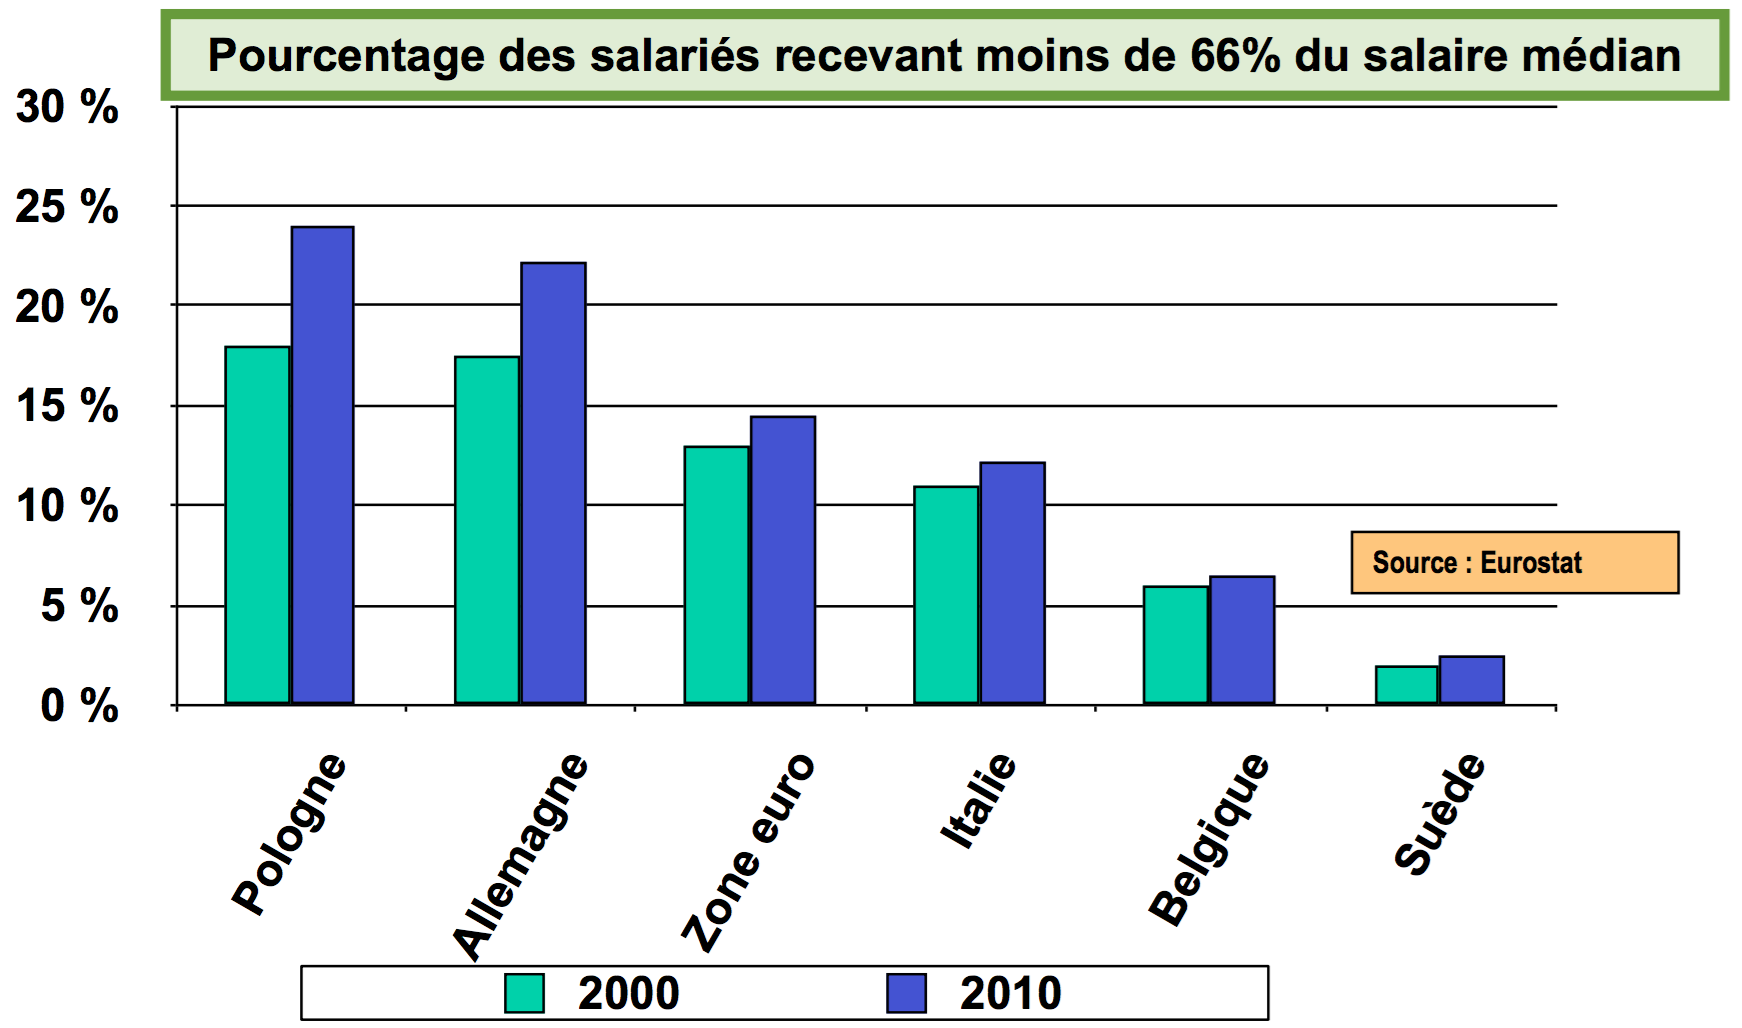
\includegraphics[scale=0.3]{64}
\end{wrapfigure}
\noindent Tout d'abord, on remarque qu'il y a une proportion de bas salaire qui est devenu plus importante qu’avant. On mesure ceci grâce au salaire médian. 50\% de la population gagne un salaire plus grand et et exactement 50\% des salaires plus bas sont gangés par l'autre moitié. On remarque que la Belgique est un peu moins bien que la Suède mais est la plus égale au niveau des salaires. Pour clarifier, pour la pologne, 24\% des gens qui ont moins de 66\% du salaire médian (donc dans tous les salarié la moitié des gens gagne moins que ce salaire et la moitié gagne plus et on prend 66\% de ce salaire).

\begin{wrapfigure}[10]{l}{9.5 cm}
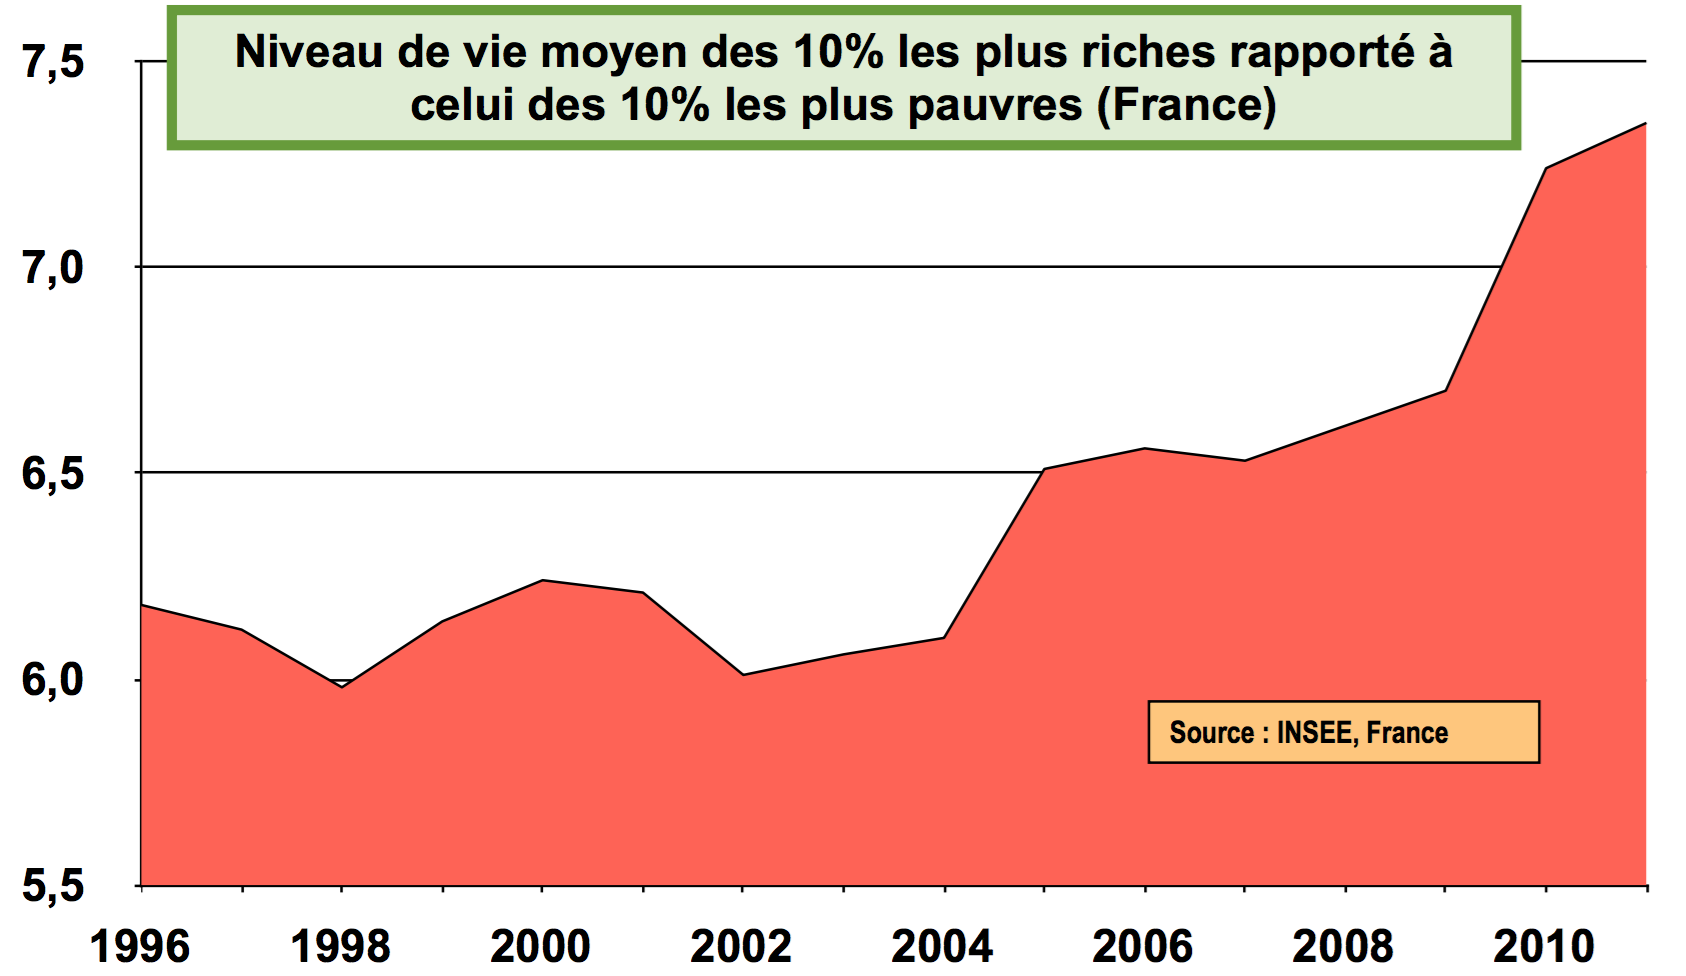
\includegraphics[scale=0.3]{65}
\end{wrapfigure}
\ \\
 Autre manière de mesurer, c’est une mesure fait en France du niveau de vie moyen des 10\% des francais qui gagne le plus par rapport au 10\% des francais qui gagne le moins. En 1996 Les plus riches gagnaient 6 fois ce que les pauvres gagnaient et maintenant on est a 7,5 fois.\\\\
On ne souhaite malgré tout pas renoncer à consommer. Les standards de vie s’élève : télévision et publicité, présence de centre commerciaux partout et présence de temps libre. Tout cela incite les gens à consommer. D'où la raison pour laquelle le low cost marche bien.

\section{Nouveaux modèles de consommation}
\subsection{Partage, location, troc, ...}
\subsubsection{Airbnb}
On en a discuté dans l'intro au chapitre. Puisque les moyens sont en baisse, on trouve de nouveaux moyens de consommer. \\
On a par exemple Airbnb qui est disponible grâce à internet et dont le concept est "Partage et location de bed \& breakfeast" entre particuliers. Et c’est beaucoup moins cher que les hôtels. 

\subsubsection{Cambio}
On a aussi Cambio (voitures partagées). On commence à voir que le pourcentage de jeune génération propriétaire d’une voiture diminue. On renonce à la propriété et on partage des véhicules. Pas encore fameux au niveau utilisation.

\subsubsection{Carpooling.com}
Ca va encore plus loin que le carsharing, c’est le covoiturage (utiliser la voiture de qq d’autre pour se déplacer). C'était déjà fortement à la mode dans les années 70' avec les prix élevés de carburants et là ça revient en force avec l'arrivée d'internet. C'est un concurrent direct pour les moyens de transport actuels puisqu'il se fait aussi à grande distance (trains, avions, bus).

\subsection{Du B2C au C2C}
Le marché traditionnel consiste en l’entreprise qui vend au consommateur. Les nouveaux marchés permettent aux consommateurs de vendre à d'autres consomateurs. On est donc plus du côté du produit recyclé que du produit nouveau. Et grâce à internet, tout cela est plus facile puisqu'on a pas besoin de marché physique. On a par exemple eBay (ventes entre particuliers), Trocheures.fr (échange de service bricolage, tu fais ce que tu sais et moi je te fait ce que je sais).

\subsection{Réaction des modèles traditionnels}
On a diférentes réactions selon le secteur concerné :
\begin{itemize}
	\item Dans l'aérien, on converge vers les nouveaux modèles low cost (on augmente le nombre de vol, de siège, utilisation de internet). Alors que les low cost évolue vers le traitionnel afin d'augmenter leur profit.

	\item Défense : TGV commence à diminuer et non a stagner donc on estime que l’impact le plus important de  baisse c’est le covoiturage. 

	\item Les consommateurs change d’attitude de plus en plus vite et donc les entreprises doivent s’adapter de plus en plus vite. Le low cost garde une longueur d'avance. 
\end{itemize}
\newpage

\section{L'avenir de l'industrie en Europe}
\subsection{Evolution de l'emploi}
On ne parlera que de la Belgique. Signalons pour commencer que beaucoup de licenciements se sont opérés dans le secteur inustriel en Belgique (ex : Caterpillar, Heinz). 
\begin{wrapfigure}[11]{l}{9.5 cm}
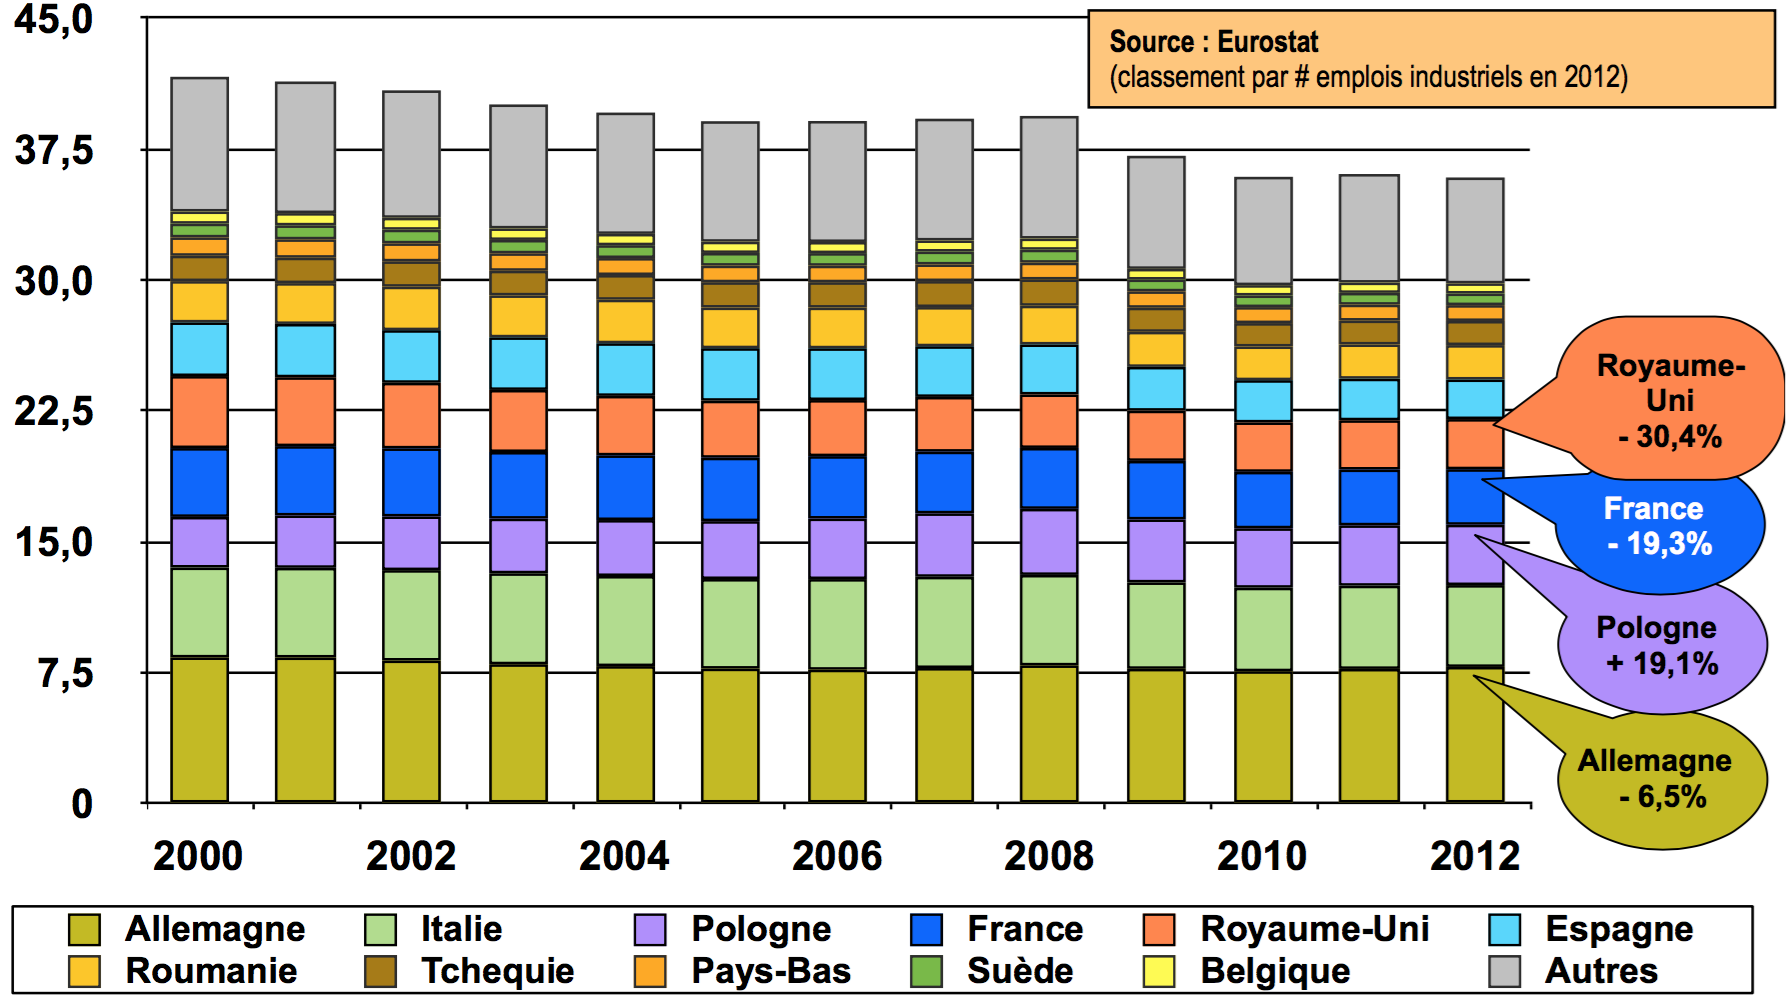
\includegraphics[scale=0.3]{66}
\end{wrapfigure}
\ \\
Pas qu'en Belgique aparemment puisque, malgré une baisse lente pendant assez longtemps, à partir de 2004 on a un véritable repli, notamment avec le UK qui a perdu 30\% d'emplois. Cas particulier de la Pologne qui doit sa hausse d'emplois à son intégration à l’UE. Tout ça correspond à 6 millions d'emploi perdus en 12 ans. 

\begin{wrapfigure}[12]{l}{9.5 cm}
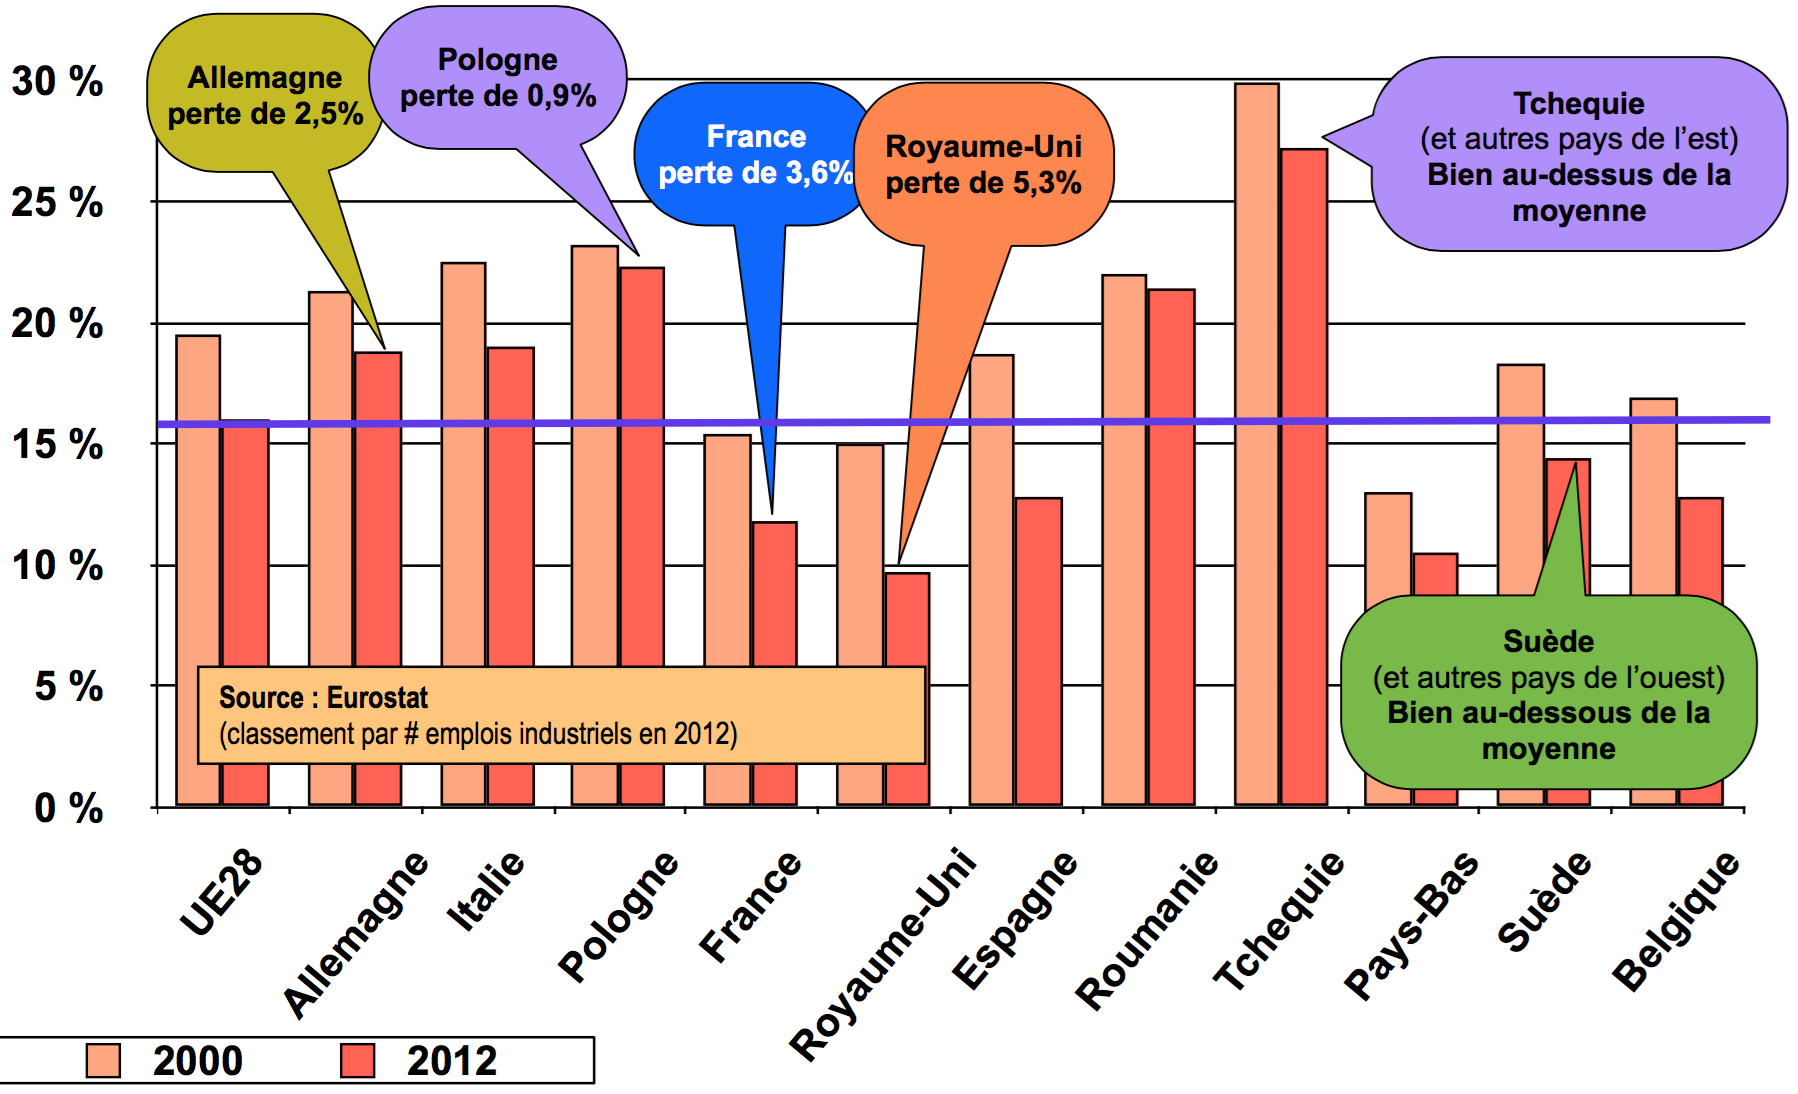
\includegraphics[scale=0.3]{67}
\end{wrapfigure}
\ \\
Sur cet autre graphe on représente la part des employés travaillant dans l'industrie. On à la barre horizontale qui représente la moyenne européenne. On peut remarquer que des pays comme la France et la Belgique sont bien en dessous et d'autres comme l'Allemagne et la Tchéquie sont bien au dessus. On remarquera qu'en générale la tendance a été une perte d'emplois dans le secteur. 

\begin{wrapfigure}[12]{l}{9.5 cm}
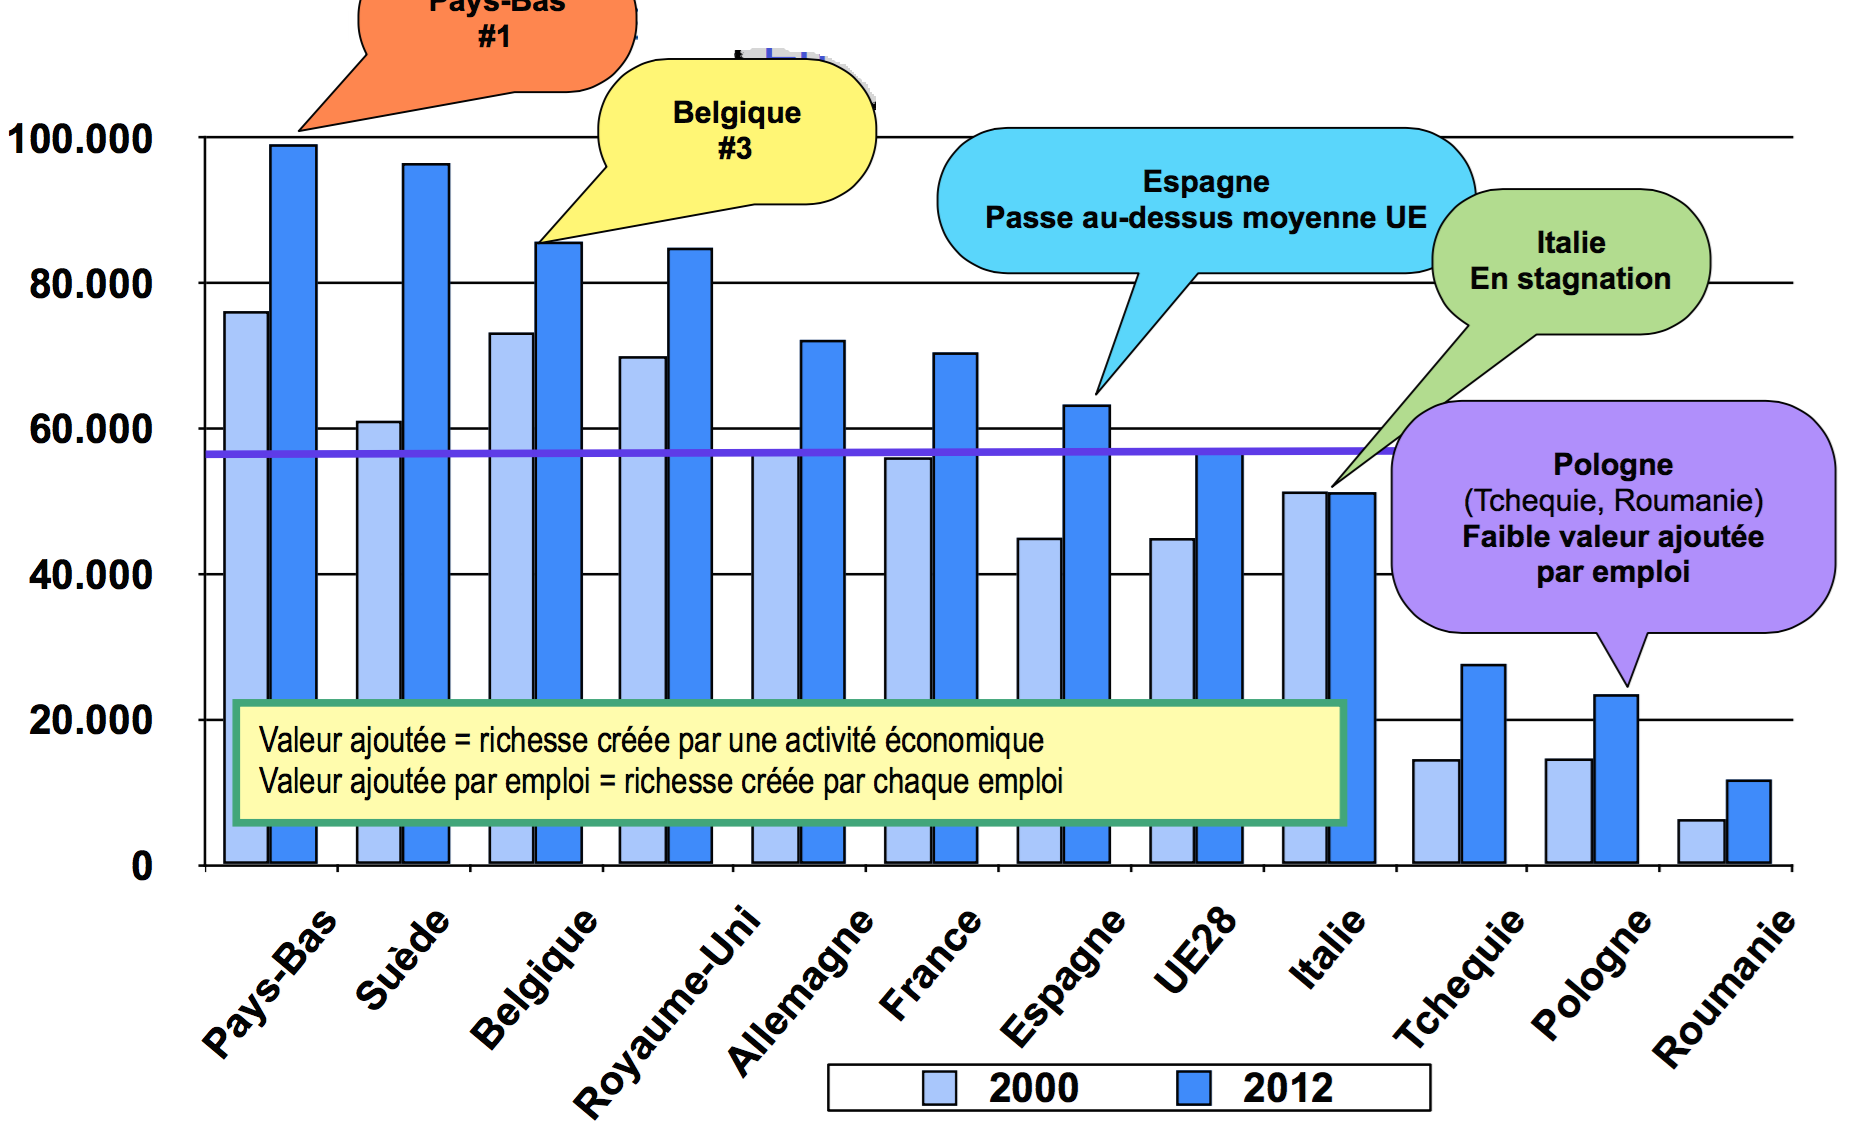
\includegraphics[scale=0.29]{68}
\end{wrapfigure}
\ \\
On parle d’industrie mais c’est pas la même chose partout. On a de l’industrie beaucoup développé et d’autres bien plus basiques. On constate que les Pays-Bas ont peu d’emplois mais chaque emploi crée beacoup de valeur. Ils ont peu d’industrie mais des industries très pointues avec des gens qualifiés. La Belgique se porte bien aussi car chaque ouvrier crée plus de valeur que ceux de l’Allemagne. On est dans une série de pays ou on est au dessus de la moyenne. Par contre les pays où il y a beaucoup d’industrie, on a très peu de valeur parce que ce sont des industries assez classiques et rudimentaires. \\
La moyenne de la part de l'industrie dans le PIB en Europe avoisine les 20\% et à part l'Allemagne et la Suède pour qui cette part est légèrement montée, cette part a baissé et en France et Belgique cette part est très basse.

\subsection{Constats}
On a une très grande disparité en Europe avec des champions comme l’Allemagne où on retrouve l’automobile haut de gamme, la téléphonie ... Là où l’Europe est forte. Dans le sud et l’est on a des produit de valeur ajoutée pas trop élevée.\\
Selon l’endroit, on a soit déclin (pays de vieille industrie comme le Benelux), soit stabilité (Allemagne, Italie), soit croissance (Europe de l'Est) de l'emploi. V slide. La croissance des pays de l’est est dû a la délocalisation. \\
La walonie est un grand exemple de la ruine de l’industrie. Mais elle s'ensort actuellement avec l’aerospatial et l'aero qui sont des points très fort de la walonie, la pharmacie et le biotech également.

\section{Exemples d'industrie}
\subsection{Lego}
Je crois qu'on sait tous ce qu'est Lego et on a tous kiffé ça ... Design, simplification et mondialisation qui ont permis la réussite de cette entreprise, née en 1980, dans le jouet Leur grande force était la petite enfance mais ils ont perdu cette activité à partir de 1998. On s’est même posé la question de savoir si lego n'avait pas raté le tournant du 21è siecle. Differentes risons : se sont trop diversifié et se sont rendu trop complexe et ont donc eu difficile à gérer tout ça. //
On a eu des baisse d’emplois importante et ils se sont dit "on a perdu cette capacité a comprendre les enfants alors on va revenir à nos racines". Ils sont reparti aux fondamentaux. Ils ont changé des choses fondamentales et depuis 2004 on travaille avec des non créateurs. Ce sont des gens qui sont nettement moins marrants mais on était obligé.
On a mis une grande priorité sur l'Asie pour la délocalisation (2008). Chaque année on a crée des produits nouveaux et ça a marché. Le siège centrale est au dannemark à billund. 

\begin{wrapfigure}[7]{l}{9.5 cm}
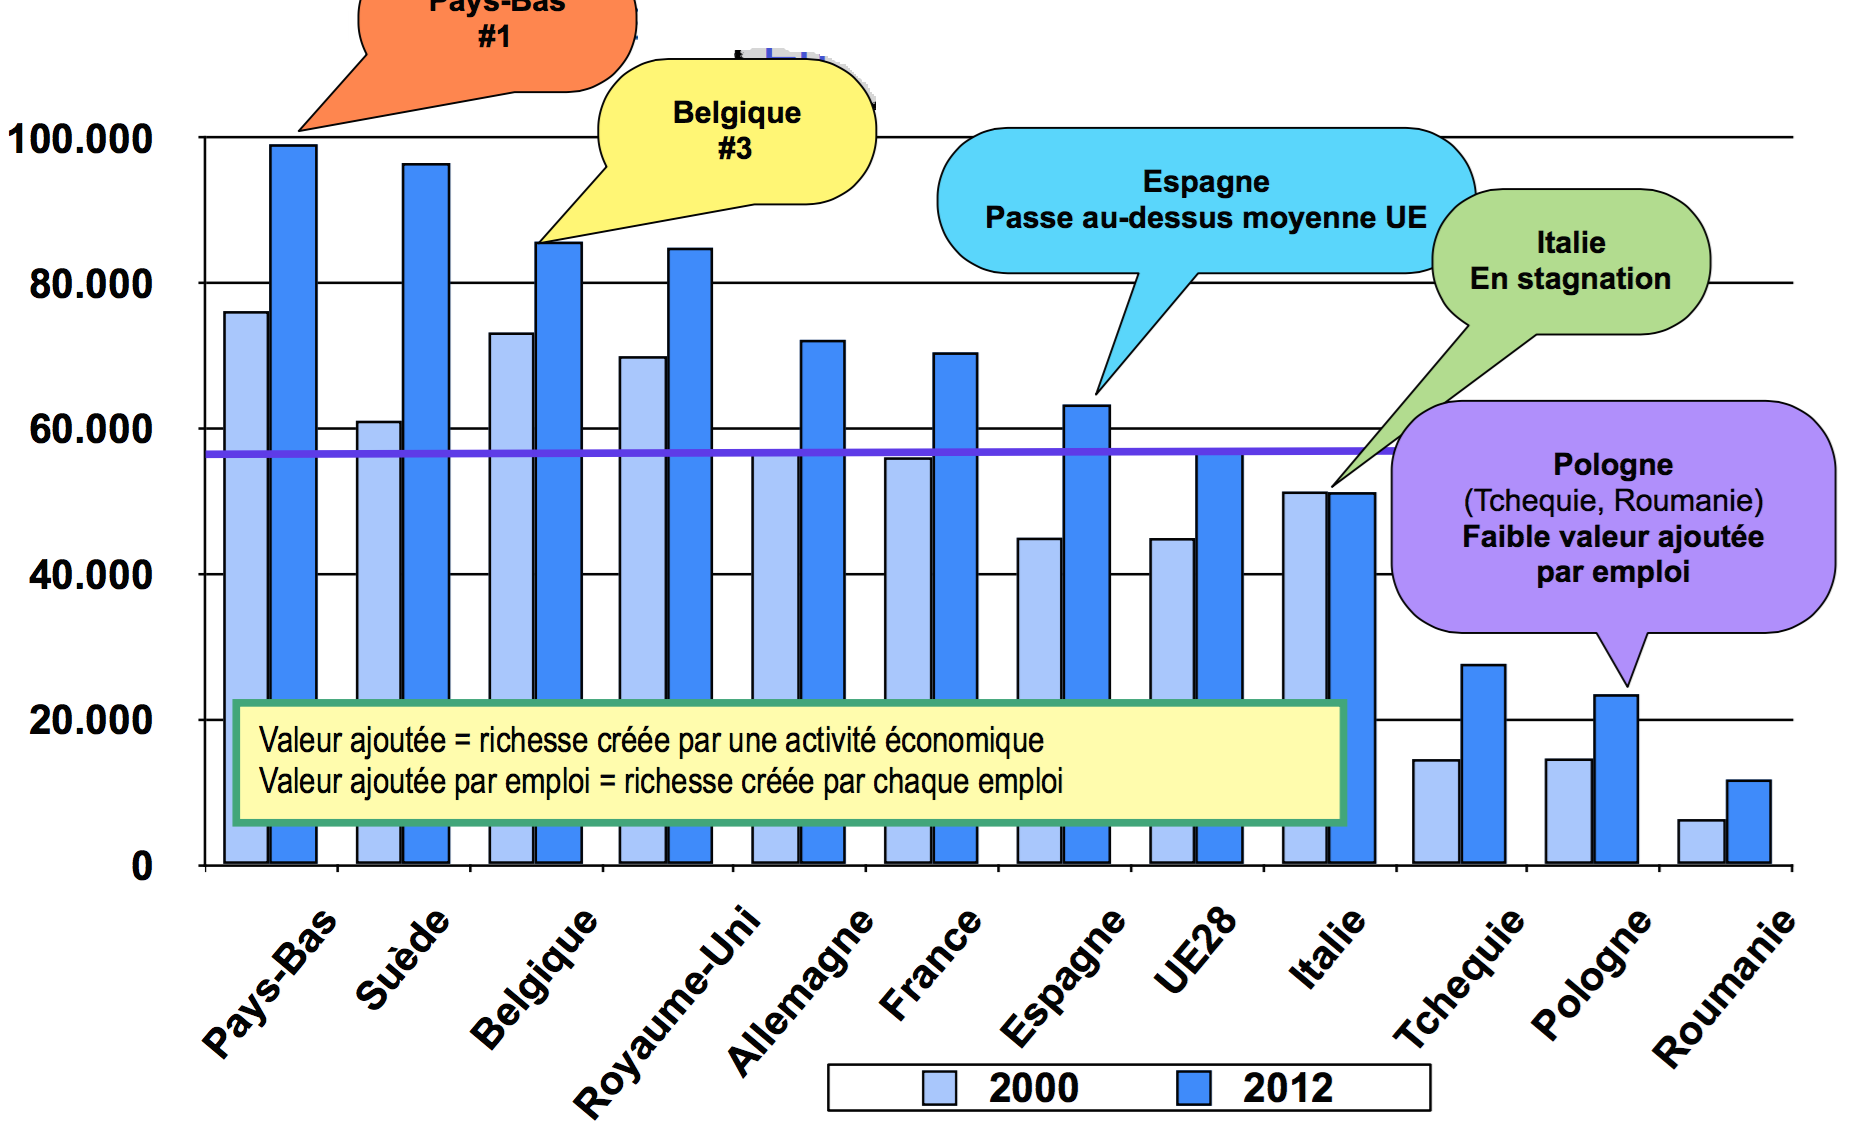
\includegraphics[scale=0.29]{68}
\end{wrapfigure}
Ils n’ont pas hésité à réduire le nombre d'employés avant de le remonter plus tard. A la base 100\% danoise puis ce sont implanté en Europe et le reste du monde. C’est un exemple réussi d’industrie mais qui a dû se remettre en question. 

\subsection{Audi Brussels}
On héberge toujours une très grande usine Audi. Ce qui a joué : gros sacrifice sociale et toujours travailler sur la qualité. Ieteren est un carossier bruxellois qui a donc débuter l'activité en 1949 en raison des droits d'importation élevés à la douane. Plein d’usines au départ. En 1975 on arrete la production de la coccinelle. Enorme croissance du groupe VW qui met en compétition ses différentes usines (vous devez etre bons en prix et en qualité). En 2005, le point positif de VW-Forest était la productivité, la qualité élevée et la localisation de l'usine (proche de frets). Fin 2005 VW récolte de mauvais résultats et décide d'une restructuration, notamment en fermant l'usine de Forest.

\subsection{SEB}
En mode fortement résumé : sacrifice sociale et qualité pour garder en vie cette société (Tefal, moulinex, krups). SEB fabrique toujours beaucoup en Europe et est protégé par des barrières technologiques. Il a massivement pratiqué l’externalisation de la production pour les bêtes produits afin de diminuer les coûts. L'entreprise mise beaucoup sur la recherche et l'innovation. 60\% des produits ont moins de 3 ans et l'équipe de recherche est assez développé. Différenciation du low cost en misant sur la sophistication (so sofisticated) et la simplicité d'usage. A partir de 2009 c'est surtout en dehors de l'Europe que les ventes ont augmentés. 

\subsection{Cardio3}
Une entreprise wallonne de biotechnologie parmi plus d’une centaine des plus grandes (GSK, UCB, IBA). 70\% de l'activité biotechnologique en Belgique ! $\pm$ 15.000 emplois industriels multiplié par 3 en 15 ans. Valorisation de la recherche universitaire. Spécialité : maladies cardiaques.

\section{Re-shoring et Back-shoring}
La mondialisation et off-shoring est une tendance longue. On observe une
 délocalisation de l’industrie européenne totale ou partielle. Totale pour les
  produits finis : textile, chaussures, meubles, électronique. Partielle : sous
  -traitance : composants, prestations, informatiques, administration, call
   centers. Pays émergents proches ou lointains. Proches : Méditerranée,
    Europe de l’est. Lointains : Asie, Amérique du Sud, . . . Afrique. Causes :
     Avantages compétitifs (Adam Smith) : Coûts salariaux (niveau de vie, 
     protection sociale, etc.) et coûts de l’énergie et des matières premières.
Délocalisation n'est pas évitable et parfois c'est totale. \\
Certains reviennent petit à petit vers leur pays d'origine. Par exemple Apple qui a rouverte une ligne de production de macbook pro aux USA et BZ Moda pour les chaussures en Italie. La cause de ce retour ? Les couts salariaux dans les pays émergents sont en train de monter alors que ceux chez nous diminuent. On a une hausse de la productivité avec la même main d’oeuvre. On est capable de s'adapter plus rapidement à toute demande et bien sûr n'oublions pas l'image de marque favorisé avec le retour au pays. \\
L'ampleur de ce reshoring est difficile à mesurer mais voici un aperçu selon
 le secteur : Textile et chaussures : 35\%, Mécanique, robotique : 20\%;
  Mobilier : 15\%; Electronique : 10\%; Electro-ménager : 10\%.

\subsection{Les leçons d'Adam Smith}
Qu’est ce qu’on a de plus que les autres ? Main d’oeuvre très qualifié, recherche … Très développé, et proximité des marchés. Désavantage : cout de la main d’oeuvre. Ils faut utiliser nos qualité en stimulant la recherche et le développement.\\
\\
Si tu es arrivé jusque là félicitation !